\input{SlideInclude.tex}

\title[Solow Model]{The Solow Model}


\begin{document}
\maketitle

\section{Production}
\begin{frame}{Production}
We assume that real GDP is produced according to
\begin{equation}
	Y_t = K_t^{\alpha} (A_tL_t)^{1-\alpha} \label{EQ_Production}
\end{equation}
where
\begin{itemize}
	\item $K_t$ is the stock of physical capital (e.g. buildings, equipment)
	\item $L_t$ is the number of workers/people
	\item $A_t$ is the level of productivity; how efficiently we use capital and labor
	\item $\alpha$ tells us how important capital is relative to labor
\end{itemize}
\end{frame}


\begin{frame}{Constant returns}
\vspace{.25in}\noindent This production function has \textbf{constant returns to scale}. If you double the rival inputs $K_t$ and $L_t$, output doubles ($A_t$ is non-rival, discussed later),
\begin{equation}
(zK_t)^{\alpha} (A_t z L_t)^{1-\alpha} = z^{\alpha}z^{1-\alpha} K_t^{\alpha} (A_tL_t)^{1-\alpha} = zY
\end{equation}
so we have constant returns because $\alpha + (1-\alpha) = 1$.
\end{frame}


\begin{frame}{GDP per capita}
GDP per capita is defined by $y_t = Y_t/L_t$. We can write this like:
\begin{eqnarray}
y_t &=& \frac{Y_t}{L_t} \nonumber \\ 
  &=& \frac{K_t^{\alpha}(A_tL_t)^{1-\alpha}}{L_t} \nonumber \\ 
  &=& \left(\frac{K_t}{A_t L_t}\right)^{\alpha} A_t \label{EQ_y_KAL}.
\end{eqnarray}
\begin{itemize}
	\item $K_t/A_tL_t$ is sometimes called ``capital per efficiency unit''. The rate of return on capital will depend on this ratio, and along a BGP this ratio will end up constant. 
	\item This means that the ``extra'' productivity term $A_t$ will drive growth in GDP per capita.
\end{itemize}

\end{frame}

\begin{frame}{The growth rate}
Take logs and derivatives of $y_t$. Start with logs:
\begin{eqnarray}
	\log y_t &=& \alpha (\log K_t/A_tL_t) + \log A_t \nonumber \\ 
	       &=& \alpha (\log K_t - \log A_t - \log L_t) + \log A_t. \label{EQ_logy}
\end{eqnarray}
and then take derivative with respect to time
\begin{equation}
	g_y = \alpha (g_K - g_A - g_L) + g_A. \label{EQ_gy}
\end{equation}

\begin{itemize}
	\item The term in parentheses represents transitory growth driven by accumulation of capital; this generates slow transitions. 
	\item The productivity growth term $g_A$ remains and drives growth along the BGP.
\end{itemize}
\end{frame}

\begin{frame}{Wages and the return to capital}
This connects to the other parts of the BGP. Assume that a large number of competitive firms in the economy produce output using the prior function, and try to maximize profits
\begin{equation}
	\pi_t = Y_t - w_tL_t - r_tK_t. \nonumber
\end{equation}
where $w_t$ is the wage and $r_t$ is the return to capital. Their first-order conditions (e.g. wage equals marginal product) are
\begin{eqnarray}
	w_t &=& \frac{\partial Y_t}{\partial L_t} = (1-\alpha)\frac{Y_t}{L_t} \nonumber \\ 
	r_t &=& \frac{\partial Y_t}{\partial K_t} = \alpha \frac{Y_t}{K_t}. \nonumber
\end{eqnarray} 
\end{frame}

\begin{frame}{Labor's share of GDP}
The first-order conditions imply
\begin{equation}
	\frac{w_tL_t}{Y_t} = 1-\alpha. \nonumber
\end{equation}
The production function is designed to ensure that labor's share of GDP is constant, to match the BGP facts.
\end{frame}

\begin{frame}{The return to capital}
From the first-order condition the return to capital is
\begin{equation}
	r_t = \frac{\alpha Y_t}{K_t}. \label{EQ_r}
\end{equation}
Along a BGP $r_t$ is constant, so it must be that $Y_t/K_t$ is constant. What's that ratio?
\begin{equation}
	\frac{Y_t}{K_t} = \frac{K_t^{\alpha}(A_tL_t)^{1-\alpha}}{K_t} = \left(\frac{A_tL_t}{K_t}\right)^{1-\alpha}. \nonumber
\end{equation}
This is what tells us that the ratio $K/AL$ must be constant along a BGP; it ensures that $r_t$ is constant along a BGP.

\end{frame}

\section{Dynamics}
\begin{frame}{Labor and Productivity}
Two of the items in the production function are assumed to just grow exogenously at a given rate. Later we'll look at what determines these growth rates.

\vspace{.25in}\noindent Labor:
\begin{equation}
	L_t = L_0 e^{g_Lt} \label{EQ_L_gL}
\end{equation}

\vspace{.25in}\noindent Productivity:
\begin{equation}
	A_t = A_0e^{g_At} \label{EQ_A_gA}
\end{equation}
\end{frame}

\begin{frame}{Capital accumulation}
Solow's model relies on one additional assumption regarding how capital accumulates:
\begin{eqnarray}
	dK &=& I_t - \delta K_t \nonumber \\ 
	   &=& s_I Y_t - \delta K_t \label{EQ_dK}
\end{eqnarray}
\begin{itemize}
	\item $dK$ is the change in the capital stock (implicitly per unit of time)
	\item $I_t$ is gross capital formation 
	\item $s_I$ is the fraction of GDP used for gross capital formation
	\item $\delta$ is the deprecation rate, the fraction of capital that breaks down each period 
\end{itemize}

\end{frame}

\begin{frame}{The growth rate of capital}
Use the accumulation and divide it by $K_t$
\begin{equation}
	g_K = s_I \frac{Y_t}{K_t} - \delta. \nonumber
\end{equation}
where $g_K = dK/K_t$ is the growth rate of capital. 

\vspace{.25in}\noindent We know $Y_t/K_t = (A_tL_t/K_t)^{1-\alpha}$ from before so
\begin{eqnarray}
	g_K &=& s_I \frac{K_t^{\alpha}(A_tL_t)^{1-\alpha}}{K_t} - \delta \nonumber \\ 
	    &=& s_I \left(\frac{A_tL_t}{K_t}\right)^{1-\alpha} - \delta. \label{EQ_gK_KAL}
\end{eqnarray}
\end{frame}

\begin{frame}{The growth rate of capital}
\begin{equation}
	g_K = s_I \left(\frac{A_tL_t}{K_t}\right)^{1-\alpha} - \delta. \label{EQ_gK_KAL}
\end{equation}
The growth rate of capital depends:
\begin{itemize}
	\item \textit{negatively} on the ratio $K_t/A_t L_t$. The bigger the stock of $K$ relative to $AL$, the slower the growth rate.
	\item \textit{positively} on $s_I$. The more resources we commit to building capital, the faster it grows.
	\item \textit{negatively} on $\delta$. The faster capital breaks down, the slower it grows.
\end{itemize}

\end{frame}

\begin{frame}{The dynamics of capital}
\begin{center}
\includegraphics[height = 3in]{../Figures/fig-ch2-fig2.eps}
\end{center}
\end{frame}

\begin{frame}{Steady state}
The dynamics ensure that the ratio evolves towards a central point where $g_K = g_A + g_L$. That point is a \textit{steady state} for $K/AL$. Solve for that ratio:
\begin{equation}
	g_A + g_L = s_I \left(\frac{AL}{K}\right)^{1-\alpha} - \delta. \nonumber
\end{equation}
which yields
\begin{equation}
	\left(\frac{K}{AL}\right)^{ss} = \left(\frac{s_I}{g_A + g_L + \delta}\right)^{\frac{1}{1-\alpha}}. \label{EQ_KAL_ss}
\end{equation}
\end{frame}

\begin{frame}{Steady state}
\begin{equation}
	\left(\frac{K}{AL}\right)^{ss} = \left(\frac{s_I}{g_A + g_L + \delta}\right)^{\frac{1}{1-\alpha}}. \label{EQ_KAL_ss}
\end{equation}
While the ratio $K/AL$ is constant at the steady state, the \textit{size} of the ratio in that steady state is
\begin{itemize}
	\item Higher when $s_I$ is large. If we commit more resources to capital accumulation, the capital stock will be relatively large in steady state.
	\item Lower when $g_L$ is large. If the population grows quickly, it is hard for capital to ``keep up'' and the ratio is lower in steady state.
	\item Lower when $g_A$ is large. If productivity grows quickly, it is also hard for capital to ``keep up''. Don't get confused, this doesn't mean productivity growth is bad for the economy.
\end{itemize}
\end{frame}

\begin{frame}{Steady state growth}
Remember that no matter what, the growth rate of GDP per capita is determined by 
\begin{equation}
	g_y = \alpha(g_K - g_A - g_L) + g_A. \nonumber
\end{equation}
THe dynamics of $K/AL$ lead to steady state where $g_K = g_A + g_L$, so
\begin{equation}
	g_y^{ss} = g_A.
\end{equation}

\begin{block}{The source of long-run growth}
In the long run the growth rate of GDP per capita is determined \textit{only} by the growth rate of productivity, $g_A$.
\end{block}
\end{frame}

\section{BGP}
\begin{frame}{Balanced growth path}
The economy ends up at a steady state. Is this steady state consistent with a balanced growth path?
\begin{itemize}
	\item The growth rate of GDP per capita is constant, $g_y^{BGP} = g_A$. \checkmark
	\item Labor's share of GDP is constant $wL/Y = 1-\alpha$. \checkmark
	\item The share of GDP used for capital accumulation is $s_I$. \checkmark
	\item The real interest rate, $r_t$, is constant. ??
\end{itemize}
\end{frame}

\begin{frame}{Real interest rate}
What's $r$? We know that
\begin{equation}
	r_t = \frac{\alpha Y_t}{K_t}. \label{EQ_r}
\end{equation}
and 
\begin{equation}
	\frac{Y_t}{K_t} = \frac{K_t^{\alpha}(A_tL_t)^{1-\alpha}}{K_t} = \left(\frac{A_tL_t}{K_t}\right)^{1-\alpha}. \nonumber
\end{equation}
so in steady state $Y/K$ is constant and
\begin{equation}
	r^{ss} = \alpha \frac{g_A + g_L + \delta}{s_I}.
\end{equation}
$r$ is constant in steady state, consistent with BGP. \checkmark
\end{frame}

\begin{frame}{Solow and BGP}
The key elements of the Solow model are
\begin{equation}
	Y_t = K_t^{\alpha} (A_tL_t)^{1-\alpha} \label{EQ_Production} \nonumber
\end{equation}
and 
\begin{equation}
	g_K = s_I \frac{Y_t}{K_t} - \delta. \nonumber
\end{equation}
which leads to:
\begin{block}{Solow and BGP}
The dynamics of capital accumulation ensure that the economy ends up in steady state, and in that steady state the economy is on a BGP.
\end{block}
\end{frame}

\begin{frame}{Other growth rates}
$K/AL$ is constant in steady state, but other important things are growing:
\begin{itemize}
	\item Total GDP. $g_Y = g_y + g_L$ so $g_Y^{ss} = g_A + g_L$
	\item Total capital. $g_K^{ss} = g_A + g_L$
	\item Consumption per capita, $c = (1-s_I)y$ so $g_c^{ss} = g_A$
	\item Capital per capita, $k = K/L$, so $g_k^{ss} = g_A$
\end{itemize}
\end{frame}

\section{Levels}
\begin{frame}{The level of GDP per capita}
The BGP is definitive about growth rates, but not the level of GDP per capita. At all times we have
\begin{equation}
	y_t = \left(\frac{K_t}{A_tL_t}\right)^{\alpha} A_t \nonumber. 
\end{equation}
so in steady state
\begin{equation}
	y_t^{BGP} = \left(\frac{s_I}{g_A + g_L + \delta}\right)^{\frac{\alpha}{1-\alpha}} A_t \label{EQ_y_BGP},
\end{equation}
and note that this still grows over time due to $A_t$ growing. 
\end{frame}

\begin{frame}{The level of GDP per capita}
We tend to think in terms of \textit{log} of GDP per capita in figures,
\begin{eqnarray}
	\log y_t^{BGP} &=& \frac{\alpha}{1-\alpha} \log \left(\frac{s_I}{g_A + g_L + \delta} \right) + \log A_t \nonumber \\ 
	     &=& \frac{\alpha}{1-\alpha} \log \left(\frac{s_I}{g_A + g_L + \delta} \right) + \log A_0 + g_A t. \label{EQ_logy_BGP} \nonumber
\end{eqnarray}
given $\log A_t = \log A_0 + g_A t$. 

\vspace{.25in}\noindent Note that this is the equation of a \textit{line}, with $\log y_t^{BGP}$ as the ``y-variable'' and $t$ as the ``x-variable''. 

\end{frame}


\begin{frame}{The level of GDP per capita}
The intercept and slope of this line:
\begin{equation}
	\log y_t^{BGP} = \underset{\text{Intercept}}{\left(\frac{\alpha}{1-\alpha} \log \left(\frac{s_I}{g_A + g_L + \delta} \right) + \log A_0\right)} + \underset{\text{Slope}}{g_A} t. \nonumber
\end{equation}
The intercept determines the level of GDP per capita along the BGP. Note that:
\begin{itemize}
	\item If $s_I$ is higher, the level of GDP p.c. is higher, even though the growth rate (slope) is not.
	\item If the initial level of productivity, $A_0$, is higher, GDP p.c. is higher, even though the growth rate (slope) is not.
\end{itemize}
\end{frame}

\section{Transitory growth}
\begin{frame}{Changes in the economy}
What happens if a parameter like $s_I$ changes? This \textit{moves} the BGP and the economy slowly adjusts until it reaches the new BGP. To understand work through distinct questions:
\begin{itemize}
	\item What happens to the dynamics of $K/AL$ immediately after the change?
	\item What happens to $K/AL$ in the long run (steady state)?
	\item What happens to the level of the BGP in response to the change?
	\item What do the $K/AL$ dynamics imply about how the economy reaches the BGP?
\end{itemize}
\end{frame}

\begin{frame}{Dynamics of $K/AL$}
If $s_I$ icnreases, $g_K$ shifts up \textit{immediately}, and the steady state is larger in the long run.
\begin{center}
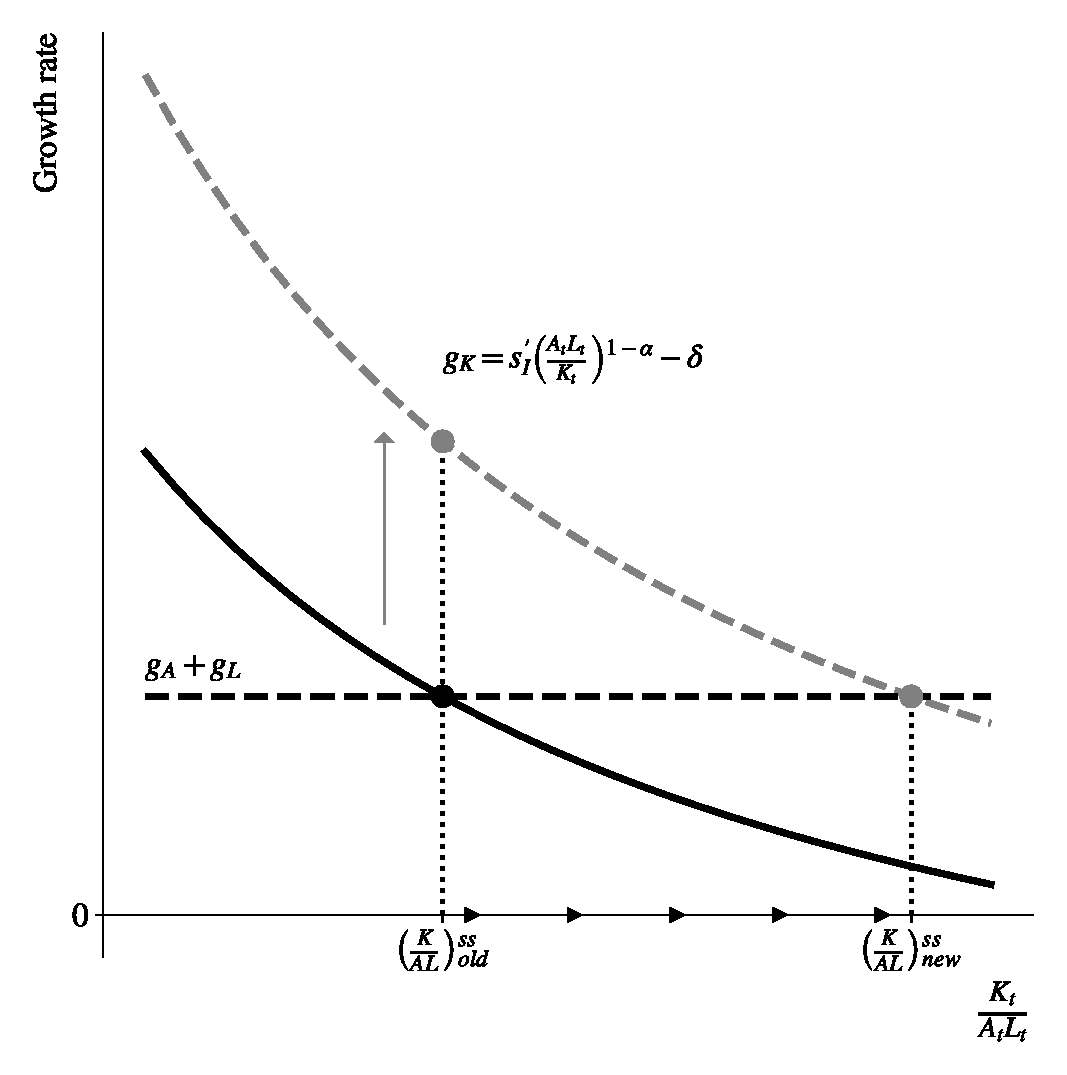
\includegraphics[height=3in]{../Figures/fig-ch2-fig3.eps}
\end{center}
\end{frame}

\begin{frame}{The growth rate}
Because $g_K$ goes up immediately, $g_y$ goes up immediately. In the long run, $g_y$ goes back to $g_A$.
\begin{center}
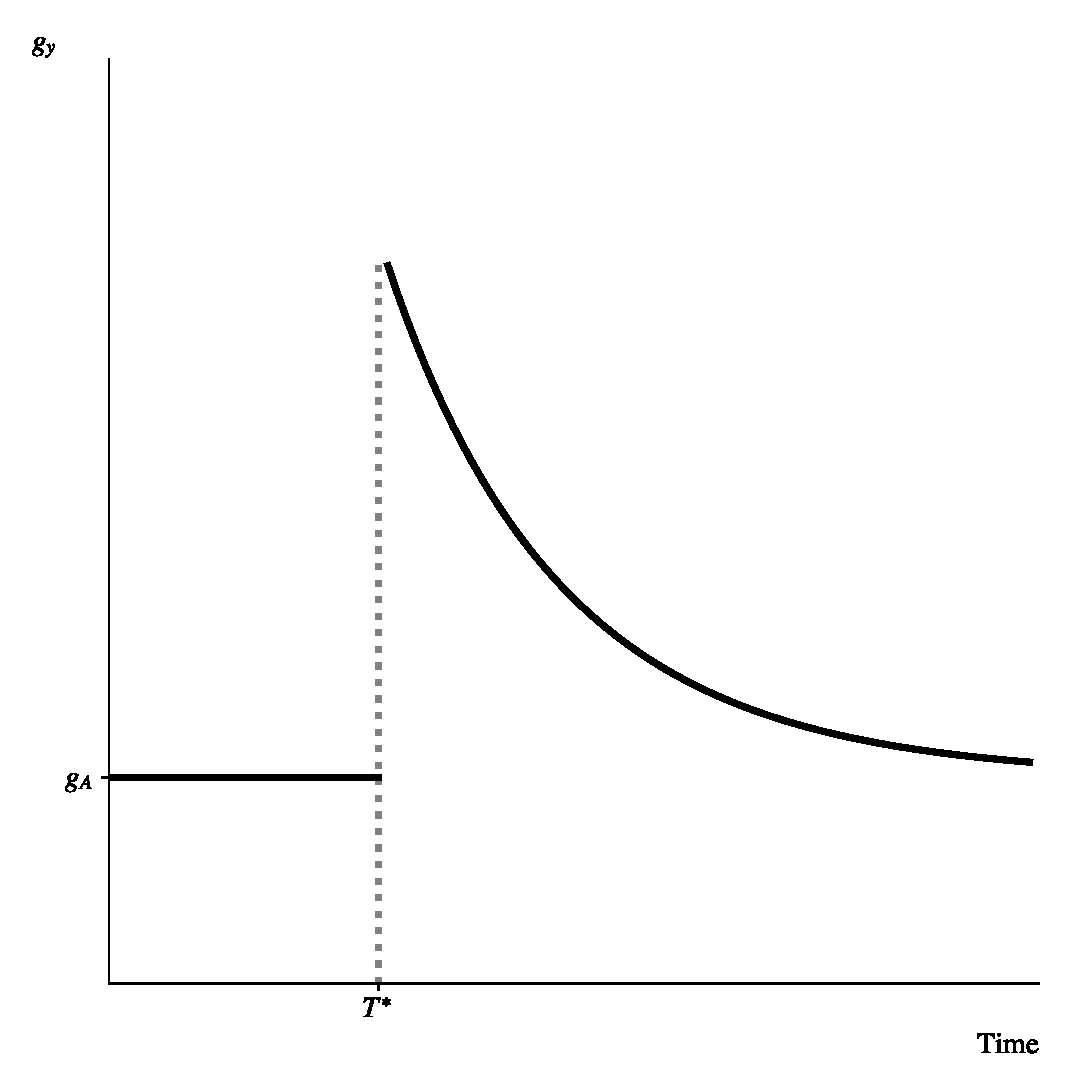
\includegraphics[height=3in]{../Figures/fig-ch2-fig4.eps}
\end{center}
\end{frame}

\begin{frame}{The level of GDP per capita}
The increase in $s_I$ shifts the BGP \textit{up}. $g_y$ implies a slow transition towards the new BGP.
\begin{center}
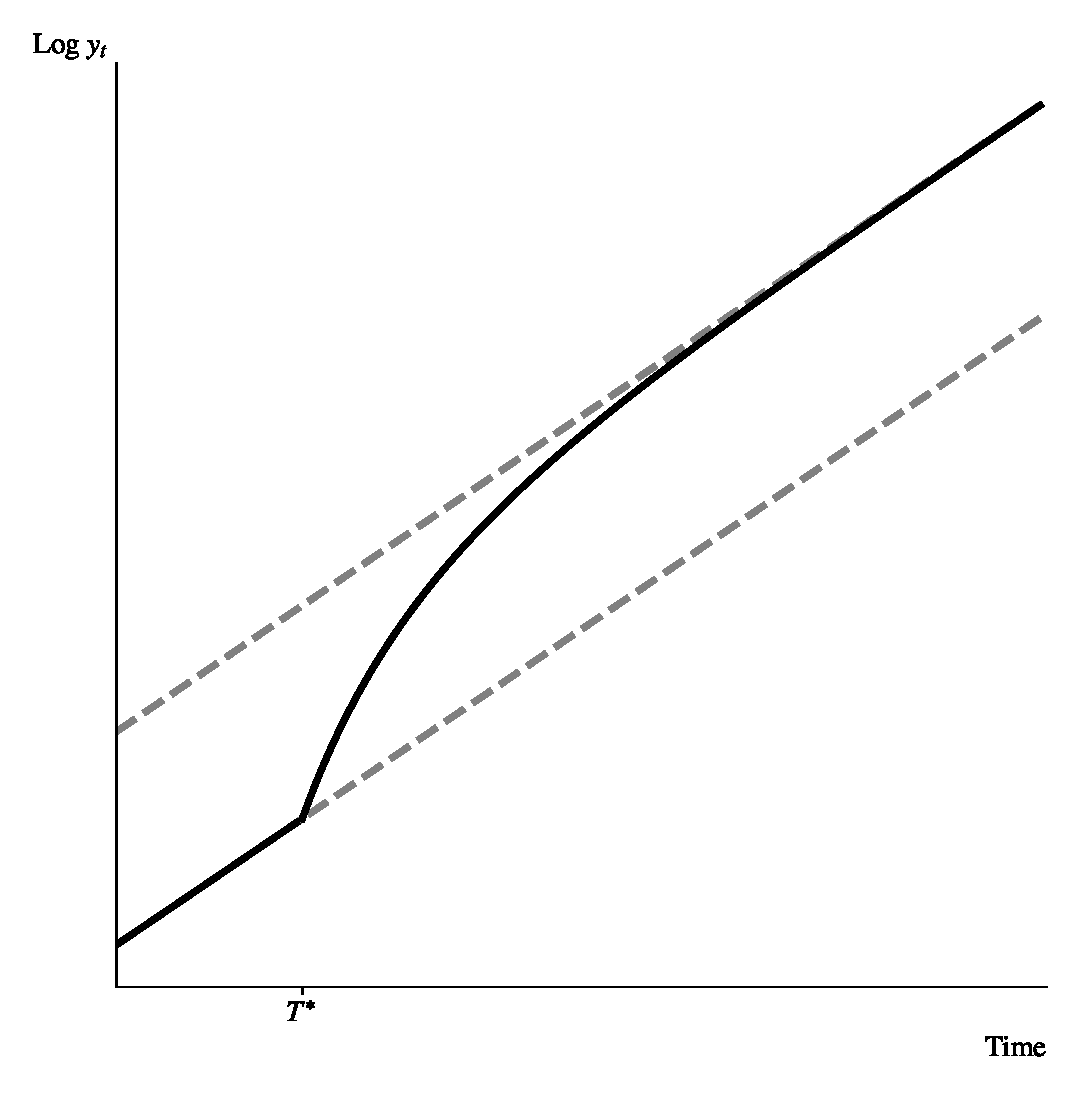
\includegraphics[height=3in]{../Figures/fig-ch2-fig5.eps}
\end{center}
\end{frame}

\begin{frame}{Transitory growth}
The increase in $s_I$ is an example of \textbf{transitory growth}. 
\begin{itemize}
	\item $g_y$ is above $g_A$ for a while, but eventually $g_y \Rightarrow g_A$
	\item Transitory growth occurs as an economy moves towards steady state
	\item This growth is transitory because the dynamics ensure that $g_K \Rightarrow g_A + g_L$
	\item Differences in growth rates across countries tend to be transitory
\end{itemize}
\vspace{.25in}\noindent
\begin{equation}
	g_y = \underset{\text{Transitory}}{\alpha (g_K - g_A - g_L)} + \underset{\text{Long-run}}{g_A} \label{EQ_gy} \nonumber
\end{equation}
\end{frame}


\end{document}